% Options for packages loaded elsewhere
\PassOptionsToPackage{unicode}{hyperref}
\PassOptionsToPackage{hyphens}{url}
%
\documentclass[
]{report}
\usepackage{amsmath,amssymb}
\usepackage{iftex}
\ifPDFTeX
  \usepackage[T1]{fontenc}
  \usepackage[utf8]{inputenc}
  \usepackage{textcomp} % provide euro and other symbols
\else % if luatex or xetex
  \usepackage{unicode-math} % this also loads fontspec
  \defaultfontfeatures{Scale=MatchLowercase}
  \defaultfontfeatures[\rmfamily]{Ligatures=TeX,Scale=1}
\fi
\usepackage{lmodern}
\ifPDFTeX\else
  % xetex/luatex font selection
\fi
% Use upquote if available, for straight quotes in verbatim environments
\IfFileExists{upquote.sty}{\usepackage{upquote}}{}
\IfFileExists{microtype.sty}{% use microtype if available
  \usepackage[]{microtype}
  \UseMicrotypeSet[protrusion]{basicmath} % disable protrusion for tt fonts
}{}
\makeatletter
\@ifundefined{KOMAClassName}{% if non-KOMA class
  \IfFileExists{parskip.sty}{%
    \usepackage{parskip}
  }{% else
    \setlength{\parindent}{0pt}
    \setlength{\parskip}{6pt plus 2pt minus 1pt}}
}{% if KOMA class
  \KOMAoptions{parskip=half}}
\makeatother
\usepackage{xcolor}
\usepackage{color}
\usepackage{fancyvrb}
\newcommand{\VerbBar}{|}
\newcommand{\VERB}{\Verb[commandchars=\\\{\}]}
\DefineVerbatimEnvironment{Highlighting}{Verbatim}{commandchars=\\\{\}}
% Add ',fontsize=\small' for more characters per line
\usepackage{framed}
\definecolor{shadecolor}{RGB}{248,248,248}
\newenvironment{Shaded}{\begin{snugshade}}{\end{snugshade}}
\newcommand{\AlertTok}[1]{\textcolor[rgb]{0.94,0.16,0.16}{#1}}
\newcommand{\AnnotationTok}[1]{\textcolor[rgb]{0.56,0.35,0.01}{\textbf{\textit{#1}}}}
\newcommand{\AttributeTok}[1]{\textcolor[rgb]{0.13,0.29,0.53}{#1}}
\newcommand{\BaseNTok}[1]{\textcolor[rgb]{0.00,0.00,0.81}{#1}}
\newcommand{\BuiltInTok}[1]{#1}
\newcommand{\CharTok}[1]{\textcolor[rgb]{0.31,0.60,0.02}{#1}}
\newcommand{\CommentTok}[1]{\textcolor[rgb]{0.56,0.35,0.01}{\textit{#1}}}
\newcommand{\CommentVarTok}[1]{\textcolor[rgb]{0.56,0.35,0.01}{\textbf{\textit{#1}}}}
\newcommand{\ConstantTok}[1]{\textcolor[rgb]{0.56,0.35,0.01}{#1}}
\newcommand{\ControlFlowTok}[1]{\textcolor[rgb]{0.13,0.29,0.53}{\textbf{#1}}}
\newcommand{\DataTypeTok}[1]{\textcolor[rgb]{0.13,0.29,0.53}{#1}}
\newcommand{\DecValTok}[1]{\textcolor[rgb]{0.00,0.00,0.81}{#1}}
\newcommand{\DocumentationTok}[1]{\textcolor[rgb]{0.56,0.35,0.01}{\textbf{\textit{#1}}}}
\newcommand{\ErrorTok}[1]{\textcolor[rgb]{0.64,0.00,0.00}{\textbf{#1}}}
\newcommand{\ExtensionTok}[1]{#1}
\newcommand{\FloatTok}[1]{\textcolor[rgb]{0.00,0.00,0.81}{#1}}
\newcommand{\FunctionTok}[1]{\textcolor[rgb]{0.13,0.29,0.53}{\textbf{#1}}}
\newcommand{\ImportTok}[1]{#1}
\newcommand{\InformationTok}[1]{\textcolor[rgb]{0.56,0.35,0.01}{\textbf{\textit{#1}}}}
\newcommand{\KeywordTok}[1]{\textcolor[rgb]{0.13,0.29,0.53}{\textbf{#1}}}
\newcommand{\NormalTok}[1]{#1}
\newcommand{\OperatorTok}[1]{\textcolor[rgb]{0.81,0.36,0.00}{\textbf{#1}}}
\newcommand{\OtherTok}[1]{\textcolor[rgb]{0.56,0.35,0.01}{#1}}
\newcommand{\PreprocessorTok}[1]{\textcolor[rgb]{0.56,0.35,0.01}{\textit{#1}}}
\newcommand{\RegionMarkerTok}[1]{#1}
\newcommand{\SpecialCharTok}[1]{\textcolor[rgb]{0.81,0.36,0.00}{\textbf{#1}}}
\newcommand{\SpecialStringTok}[1]{\textcolor[rgb]{0.31,0.60,0.02}{#1}}
\newcommand{\StringTok}[1]{\textcolor[rgb]{0.31,0.60,0.02}{#1}}
\newcommand{\VariableTok}[1]{\textcolor[rgb]{0.00,0.00,0.00}{#1}}
\newcommand{\VerbatimStringTok}[1]{\textcolor[rgb]{0.31,0.60,0.02}{#1}}
\newcommand{\WarningTok}[1]{\textcolor[rgb]{0.56,0.35,0.01}{\textbf{\textit{#1}}}}
\usepackage{longtable,booktabs,array}
\usepackage{calc} % for calculating minipage widths
% Correct order of tables after \paragraph or \subparagraph
\usepackage{etoolbox}
\makeatletter
\patchcmd\longtable{\par}{\if@noskipsec\mbox{}\fi\par}{}{}
\makeatother
% Allow footnotes in longtable head/foot
\IfFileExists{footnotehyper.sty}{\usepackage{footnotehyper}}{\usepackage{footnote}}
\makesavenoteenv{longtable}
\usepackage{graphicx}
\makeatletter
\def\maxwidth{\ifdim\Gin@nat@width>\linewidth\linewidth\else\Gin@nat@width\fi}
\def\maxheight{\ifdim\Gin@nat@height>\textheight\textheight\else\Gin@nat@height\fi}
\makeatother
% Scale images if necessary, so that they will not overflow the page
% margins by default, and it is still possible to overwrite the defaults
% using explicit options in \includegraphics[width, height, ...]{}
\setkeys{Gin}{width=\maxwidth,height=\maxheight,keepaspectratio}
% Set default figure placement to htbp
\makeatletter
\def\fps@figure{htbp}
\makeatother
\setlength{\emergencystretch}{3em} % prevent overfull lines
\providecommand{\tightlist}{%
  \setlength{\itemsep}{0pt}\setlength{\parskip}{0pt}}
\setcounter{secnumdepth}{5}
\usepackage{booktabs}
\usepackage{booktabs}
\usepackage{longtable}
\usepackage{array}
\usepackage{multirow}
\usepackage{wrapfig}
\usepackage{float}
\usepackage{colortbl}
\usepackage{pdflscape}
\usepackage{tabu}
\usepackage{threeparttable}
\usepackage{threeparttablex}
\usepackage[normalem]{ulem}
\usepackage{makecell}
\usepackage{xcolor}
\ifLuaTeX
  \usepackage{selnolig}  % disable illegal ligatures
\fi
\usepackage[]{natbib}
\bibliographystyle{apalike}
\IfFileExists{bookmark.sty}{\usepackage{bookmark}}{\usepackage{hyperref}}
\IfFileExists{xurl.sty}{\usepackage{xurl}}{} % add URL line breaks if available
\urlstyle{same}
\hypersetup{
  pdftitle={A Book Chapter Example},
  pdfauthor={Your Name},
  hidelinks,
  pdfcreator={LaTeX via pandoc}}

\title{A Book Chapter Example}
\author{Your Name}
\date{}

\usepackage{amsthm}
\newtheorem{theorem}{Theorem}[chapter]
\newtheorem{lemma}{Lemma}[chapter]
\newtheorem{corollary}{Corollary}[chapter]
\newtheorem{proposition}{Proposition}[chapter]
\newtheorem{conjecture}{Conjecture}[chapter]
\theoremstyle{definition}
\newtheorem{definition}{Definition}[chapter]
\theoremstyle{definition}
\newtheorem{example}{Example}[chapter]
\theoremstyle{definition}
\newtheorem{exercise}{Exercise}[chapter]
\theoremstyle{definition}
\newtheorem{hypothesis}{Hypothesis}[chapter]
\theoremstyle{remark}
\newtheorem*{remark}{Remark}
\newtheorem*{solution}{Solution}
\begin{document}
\maketitle

{
\setcounter{tocdepth}{1}
\tableofcontents
}
\hypertarget{an-introduction-to-nonparametric-methods-schistosomiasis}{%
\chapter{An Introduction to Nonparametric Methods: Schistosomiasis}\label{an-introduction-to-nonparametric-methods-schistosomiasis}}

\emph{Using statistics is no substitute for thinking about the problem}
-Douglas Montgomery\footnote{Douglas Montgomery, Design and Analysis of Experiments, Fifth edition, Wiley, 2003, page 21.}

Randomization tests, permutation tests, and bootstrap methods are quickly gaining in popularity as methods for conduct statistical inference. Why? These nonparametric methods require fewer assumptions and provide results that are often more accurate than those from traditional techniques using well-known distributions (such as the normal, t, or F distribution). These methods are based on computer simulations instead of distributional assumptions and thus are particularly useful when the sample data are skewed or if the sample size is small. In addition, nonparametric methods can be extended to other parameters of interest, such as the median or standard deviation, while the well known parametric methods described in introductory statistics courses are often restricted to just inference for the population mean.

~~~~We begin this chapter by comparing two treatments for a potentially deadly disease called Schistosomiasis (shis-tuh-soh-mahy-uh-sis). We illustrate the basic concepts behind nonparametric methods by using randomization tests to:

\begin{itemize}
\tightlist
\item
  Provide an intuitive description of statistical inference.
\item
  Conduct a randomization test by hand
\item
  Use software to conduct a randomization test
\item
  Compare one-sided and two-sided hypothesis tests
\item
  Making connections between randomization tests and conventional terminology
\end{itemize}

After working through the schistosomiasis investigation, you will have the opportunity to
analyze several other data sets using randomization tests, permutation tests, bootstrap methods,
and rank-based nonparametric tests.

\hypertarget{investigation-can-a-new-drug-reduce-the-spread-of-schistosomiasis}{%
\section{\texorpdfstring{\textbf{Investigation: Can a New Drug Reduce the Spread of Schistosomiasis?}}{Investigation: Can a New Drug Reduce the Spread of Schistosomiasis?}}\label{investigation-can-a-new-drug-reduce-the-spread-of-schistosomiasis}}

Schistosomiasis is a disease occurring in humans caused by parasitic flatworms called schistosomes (skis'-tuhsohms).
Schistosomiasis affects about 200 million people worldwide and is a serious problem in sub-Saharan
Africa, South America, China, and Southeast Asia. The disease can cause death, but more commonly results
in chronic and debilitating symptoms, arising primarily from the body's immune reaction to parasite eggs
lodged in the liver, spleen, and intestines.

~Currently there is one drug, praziquantel (prā'zĭ-kwän'těl'), in common use for treatment of schistosomiasis; it is cheap and effective. However many organizations are worried about relying on a single drug to treat a serious disease which affects so many people worldwide. Drug resistance may have prompted a 1990s outbreak in Senegal, where cure rates were low. In 2007, several researchers published work involving a promising drug called K11777 that, in theory, might also treat schistosomiasis.

~In this chapter, we will analyze data from this study where the researchers wanted to find out whether K11777 helps to stop schistosome worms from growing. In one phase of the study, 10 female laboratory mice and 10 male laboratory mice were deliberately infected with the schistosome parasite. Seven days after being infected with schistosomiasis, each mouse was given injections every day for 28 days. Within each sex, 5 mice were randomly assigned to a treatment of K11777 whereas the other 5 mice formed a control group injected with an equal volume of plain water. At day 49, the researchers euthanized the mice and measured both the number of eggs and the numbers of worms in the mice livers. Both numbers were expected to be lower if the drug was effective.

Table 1.1 gives the worm count for each mouse. An individual value plot of the data is shown in Figure 1.1. Notice that the treatment group has fewer worms than the control group for both females and males.

\begin{table}[!h]
\centering
\caption{\label{tab:table1}Worm count data for the schistosomiasis study. Treatment is a regimen of K11777 injections from day 7 to day 35. Control is the same regimen, but with a water solution only.}
\centering
\fontsize{10}{12}\selectfont
\begin{tabular}[t]{lrrr}
\toprule
\multicolumn{2}{c}{Female} & \multicolumn{2}{c}{Male} \\
\cmidrule(l{3pt}r{3pt}){1-2} \cmidrule(l{3pt}r{3pt}){3-4}
Treatment & Control & Treatment & Control\\
\midrule
\cellcolor{gray!10}{1} & \cellcolor{gray!10}{16} & \cellcolor{gray!10}{3.0} & \cellcolor{gray!10}{31}\\
2 & 10 & 5.0 & 26\\
\cellcolor{gray!10}{2} & \cellcolor{gray!10}{10} & \cellcolor{gray!10}{9.0} & \cellcolor{gray!10}{28}\\
10 & 7 & 10.0 & 13\\
\cellcolor{gray!10}{7} & \cellcolor{gray!10}{17} & \cellcolor{gray!10}{6.0} & \cellcolor{gray!10}{47}\\
\addlinespace
\textbf{Mean 4.4} & \textbf{12} & \textbf{6.6} & \textbf{29}\\
\bottomrule
\end{tabular}
\end{table}

\begin{figure}
\centering
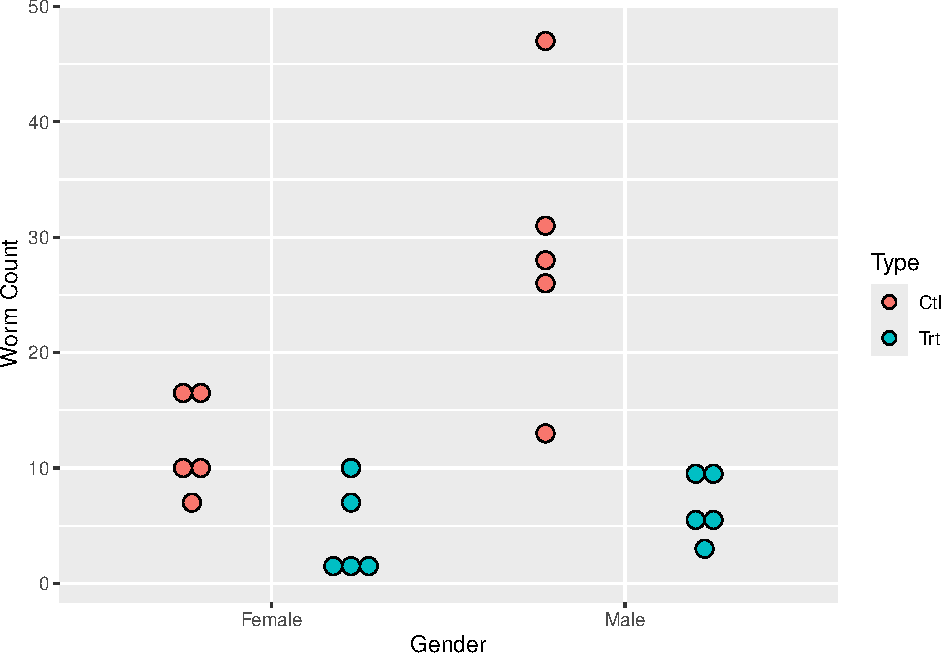
\includegraphics{index_files/figure-latex/graph1-1.pdf}
\caption{\label{fig:graph1}Individual value plot of the worm count data}
\end{figure}

\newpage

\begin{quote}
\textbf{NOTE}
There is a difference between individual value plots and dotplots. In dotplots (such as Figures 1.3 and
1.4 shown later in this chapter), each observation is represented by a dot along a number line (x-axis).
When values are close or the same, the dots are stacked. Dotplots can be used in place of histograms
when the sample size is small. Individual value plots, as shown in Figure 1.1, are used to simultaneously
display each observation for multiple groups. They can be used instead of boxplots to identify outliers and distribution shape, especially when there are relatively few observations.
\end{quote}

\hypertarget{activity-describing-the-data}{%
\section*{\texorpdfstring{Activity: \emph{Describing the Data}}{Activity: Describing the Data}}\label{activity-describing-the-data}}
\addcontentsline{toc}{section}{Activity: \emph{Describing the Data}}

\begin{quote}
\begin{enumerate}
\def\labelenumi{\arabic{enumi}.}
\tightlist
\item
  Use Figure 1.1 to visually compare the number of worms for the treatment and control groups for both
  the male and the female mice. Does each of the four groups appear to have a similar center and a similar
  spread? Are there any outliers (extreme observations that don't seem to fit with the rest of the data)?
\item
  Calculate appropriate summary statistics (e.g., the median, mean, standard deviation, and range) for
  each of the four groups. For the female mice, calculate the difference between the treatment and control
  group means. Do the same for the male mice.
\end{enumerate}
\end{quote}

The descriptive analysis in Questions 1 and 2 points to a positive treatment effect: K11777 appears to have

reduced the number of parasitic worms in this sample. But descriptive analysis is usually only the first step
in ascertaining whether an effect is real; we often conduct a significance test or create a confidence interval
to determine if chance alone could explain the effect.

Most introductory statistics courses focus on hypothesis tests that involve using a normal, t-, chi-square or F-distribution to calculate the p-value. These tests are often based on the central limit theorem. In the

schistosomiasis study, there are only five observations in each group. This is a much smaller sample size
than is recommended for the central limit theorem, especially given that Figure 1.1 indicates that the data
may not be normally distributed. Since we cannot be confident that the sample averages are normally distributed,
we will use a distribution-free test, also called a nonparametric test. Such tests do not require
the distribution of our sample statistic to have any specific form and are often useful in studies with very
small sample sizes.

\large

\textbf{MATHEMATICAL NOTE:}
For any population with mean m and finite standard deviation s, the central limit theorem states that
the sample mean x from an independent and identically distributed sample tends to follow the normal
distribution if the sample size is large enough. The mean of x is the same as the population mean, m, while
the standard deviation of x is s/1n, where n is the sample size.

\normalsize

We will use a form of nonparametric statistical inference known as a randomization hypothesis test to analyze the data from the schistosomiasis study. \textbf{Randomization hypothesis} tests are significance tests that simulate the random allocation of units to treatments many times in order to determine the likelihood of observing an outcome at least as extreme as the one found in the actual study.

\Large

\textbf{\textcolor{red}{Key Concept:}}
\textcolor{red}{\textbf{Parametric tests} (such as $z$-tests, $t$-tests, or $F$-tests) assume that data come from a population that follows a probability distribution or use the central limit theorem to make inferences about a population. \textbf{Nonparametric tests} (such as randomization tests) do not require assumptions about the distribution of the population or large sample sizes in order to make inferences about a population.}

\normalsize

We will introduce the basic concepts of randomization tests in a setting where units (mice in this example) are randomly allocated to a treatment or control group. Using a significance test, we will decide if an observed treatment effect (the observed difference between the mean responses in the treatment and control) is ``real'' or if ``random chance alone'' could plausibly explain the observed effect. The null hypothesis states that ``random chance alone'' is the reason for the observed effect. In this initial discussion, the alternative hypothesis will be onesided because we want to show that the true treatment mean (\(\mu\)treatment) is less than the true control mean (\(\mu\)control). Later, we will expand the discussion to consider modifications needed to deal with two-sided alternatives.

\hypertarget{statistical-inference-through-a-randomization-test}{%
\section{\texorpdfstring{\textbf{Statistical Inference Through a Randomization Test}}{Statistical Inference Through a Randomization Test}}\label{statistical-inference-through-a-randomization-test}}

Whether they take the form of significance tests or confidence intervals, inferential procedures rest on the fundamental question for inference: ``What would happen if we did this many times?'' Let's unpack this
question in the context of the female mice in the schistosomiasis study. We observed a difference in means
of 7.6 = 12.00 - 4.40 worms between control and treatment groups. While we expect that this large difference
reflects the effectiveness of the drug, it is possible that chance alone could explain this difference. This
``chance alone'' position is usually called the null hypothesis and includes the following assumptions:

\begin{itemize}
\tightlist
\item
  The number of parasitic worms found in the liver naturally varies from mouse to mouse.
\item
  Whether or not the drug is effective, there clearly is variability in the responses of mice to the infestation
  of schistosomes.
\item
  Each group exhibits this variability, and even if the drug is not effective, some mice do better than
  others.
\item
  The only explanation for the observed difference of 7.6 worms in the means is that the random
  allocation randomly placed mice with larger numbers of worms in the control group and mice with
  smaller numbers of worms in the treatment group.
\end{itemize}

In this study, the null hypothesis is that the treatment has no effect on the average worm count, and it

is denoted as
\textbar{} \(H_0\): \(\mu\)control = \(\mu\)treatment
Another way to write this null hypothesis is
\(H_0\): the treatment has no effect on average worm count

The research hypothesis (the treatment causes a reduction in the average worm count) is called the alternative
hypothesis and is denoted \(H_a\) (or \(H_1\)). For example,
\(H_a\): mcontrol 7 mtreatment
Another way to write this alternative hypothesis is
Ha: the treatment reduces the average worm count
Alternative hypotheses can be ``one-sided, greater than'' (as in this investigation), ``one-sided, less-than''
(the treatment causes an increase in worm count), or ``two-sided'' (the treatment mean is different, in one
direction or the other, from the control mean). We chose to test a one-sided hypothesis because there is a
clear research interest in one direction. In other words, we will take action (start using the drug) only if we
can show that K11777 reduces the worm count.

\Large

\textbf{\textcolor{red}{Key Concept:}}
\textcolor{red}{\textbf{The fundamental question for inference}: Every statistical inference procedure (parametric or nonparametric) is based on the question “How does what we observed in our data compare to what
would happen if the null hypothesis were actually true and we repeated the process many times?”
For a randomization test comparing responses for two groups, this question becomes “How does
the observed difference between groups compare to what would happen if the treatments actually
had no effect on the individual responses and we repeated the random allocation of individuals to
groups many times?”}

\normalsize

\hypertarget{activity-conducting-a-randomization-test-by-hand}{%
\section*{\texorpdfstring{Activity: \emph{Conducting a Randomization Test by Hand}}{Activity: Conducting a Randomization Test by Hand}}\label{activity-conducting-a-randomization-test-by-hand}}
\addcontentsline{toc}{section}{Activity: \emph{Conducting a Randomization Test by Hand}}

\begin{enumerate}
\def\labelenumi{\arabic{enumi}.}
\setcounter{enumi}{2}
\tightlist
\item
  To get a feel for the concept of a p-value, write each of the female worm counts on an index card.
  Shuffle the 10 index cards, and then draw five cards at random (without replacement). Call these five
  cards the treatment group and the five remaining cards the control group. Under the null hypothesis
  (i.e.~the treatment has no effect on worm counts), this allocation mimics precisely what actually happened
  in our experiment, since the only cause of group differences is the random allocation.
  \textbar{} Calculate the mean of the five cards representing the treatment group and the mean of the five
  cards representing the control group. Then find the difference between the control and treatment group means that you obtained in your allocation. To be consistent, take the control group mean minus the
  treatment group mean. Your work should look similar to the following simulation:
\end{enumerate}

{[}{[}{[}Fig\_CT{]}{]}{]}

\begin{enumerate}
\def\labelenumi{\arabic{enumi}.}
\setcounter{enumi}{3}
\item
  If you were to do another random allocation, would you get the same difference in means? Explain.
\item
  Now, perform nine more random allocations, each time computing and writing down the difference in
  mean worm count between the control group and the treatment group. Make a dotplot of the 10 differences.
  What proportion of these differences are 7.6 or larger?
\item
  If you performed the simulation many times, would you expect a large percentage of the simulations to
  result in a mean difference greater than 7.6? Explain.
\end{enumerate}

The reasoning in the previous activity leads us to the randomization test and an interpretation of the

fundamental question for inference. The fundamental question for this context is as follows: ``If the null
hypothesis were actually true and we randomly allocated our 10 mice to treatment and control groups many
times, what proportion of the time would the observed difference in means be as big as or bigger than 7.6?''
This long-run proportion is a probability that statisticians call the \textbf{p-value} of the randomization test. The
p-values for most randomization tests are found through simulations. Despite the fact that simulations do
not give exact p-values, they are usually preferred over the tedious and time-consuming process of listing
all possible outcomes. Researchers usually pick a round number such as 10,000 repetitions of the simulation
and approximate the p-value accordingly. Since this p-value is an approximation, it is often referred to as
the \textbf{empirical p-value}.

\Large

\textbf{\textcolor{red}{Key Concept:}}
\textcolor{red}{Assuming that nothing except the random allocation process is creating group differences, the p-value
of a randomization test is the probability of obtaining a group difference as large as or larger than
the group difference actually observed in the experiment.}

\Large

\textbf{\textcolor{red}{Key Concept:}}

\textcolor{red}{The calculation of an empirical p-value requires these steps:
\begin{itemize}
\item Repeat the random allocation process a number of times (N times).
\item Record, each time, whether or not the group difference exceeds or is the same as the one
observed in the actual experiment (let X be the number of times the group difference exceeds
or is the same as the one observed).
\item Compute X/N to get the p-value, the proportion of times the difference exceeds or is the same
as the observed difference.
\end{itemize}}

\large

\textbf{NOTE:}
Many researchers include the observed value as one of the possible outcomes. In this case, N = 9999
iterations are typically used and the p-value is calculated as (X + 1)/(9999 + 1). The results are very
similar whether X/10,000 or (X + 1)/(9999 + 1) is used. Including the observed value as one of the
possible allocations is a more conservative approach and protects against getting a p-value of 0. Our
observation from the actual experiment provides evidence that the true p-value is greater than zero.

\hypertarget{performing-a-randomization-test-using-a-computer-simulation}{%
\section{\texorpdfstring{\textbf{Performing a Randomization Test Using a Computer Simulation}}{Performing a Randomization Test Using a Computer Simulation}}\label{performing-a-randomization-test-using-a-computer-simulation}}

\normalsize

While physical simulations (such as the index cards activity) help us understand the process of computing an
empirical p-value, using computer software is a much more efficient way of producing an empirical p-value
based on a large number of iterations. If you are simulating 10 random allocations, it is just as easy to use index cards as a computer. However, the advantage of a computer simulation is that 10,000 random allocations
can be conducted in almost the same amount of time it takes to simulate 10 allocations. In the following
steps, you will develop a program to calculate an empirical p-value.

\hypertarget{activity-using-computer-simulations-to-conduct-a-hypothesis-test}{%
\section*{\texorpdfstring{Activity: \emph{Using Computer Simulations to Conduct a Hypothesis Test}}{Activity: Using Computer Simulations to Conduct a Hypothesis Test}}\label{activity-using-computer-simulations-to-conduct-a-hypothesis-test}}
\addcontentsline{toc}{section}{Activity: \emph{Using Computer Simulations to Conduct a Hypothesis Test}}

\begin{enumerate}
\def\labelenumi{\arabic{enumi}.}
\setcounter{enumi}{6}
\item
  Use the technology instructions provided on the CD to insert the schistosomiasis data into a statistical
  software package and randomly allocate each of the 10 female worm counts to either the treatment or the
  control group.
\item
  Take the control group average minus the K11777 treatment group average.
\item
  Use the instructions to write a program, function, or macro to repeat the process 10,000 times. Count
  the number of simulations where the difference between the group averages (control minus K11777) is
  greater than or equal to 7.6, divide that count by 10,000, and report the resulting empirical p-value.
\item
  Create a histogram of the 10,000 simulated differences between group means and comment on the
  shape of the histogram. This histogram, created from simulations of a randomization test, is called an
  empirical randomization distribution. This distribution describes the frequency of each observed
  difference (between the control and treatment means) when the null hypothesis is true.
\item
  Based on your results in Questions 9 and 10 and assuming the null hypothesis is true, about how frequently
  do you think you would obtain a mean difference as large as or larger than 7.6 by random allocation alone?
\item
  Does your answer to Question 11 lead you to believe the ``chance alone'' position (i.e., the null hypothesis
  that the mean worm count is the same for both the treatment and the control), or does it lead you to
  believe that K11777 has a positive inhibitory effect on the schistosome worm in female mice? Explain.
\end{enumerate}

Figure 1.2 shows a histogram resulting from the previous activity. A computer simulation of Question 9

resulted in a p-value of 281/10,000 = 0.0281. This result shows that random allocation alone would produce
a mean group difference as large as or larger than 7.6 only about 3\% of the time, suggesting that something
other than chance is needed to explain the difference in group means. Since the only other distinction between
the groups is the presence or absence of treatment, we can conclude that the treatment causes a reduction in
worm counts.

We conducted four more simulations, each with 10,000 iterations, which resulted in p-values of 0.0272,

0.0282, 0.0268, and 0.0285. When the number of iterations is large, the empirical randomization distribution
(such as the histogram created in Question 10) provides a precise estimate of the likelihood of all possible values of the difference between the control and treatment means. Thus, when the number of iterations is large,
well-designed simulation studies result in empirical p-values that are fairly accurate. The larger the number
of iterations (i.e., randomizations) within a simulation study, the more precise the p-value is.

{[}{[}{[}Fig1.2{]}{]}{]}

~Because the sample sizes in the schistosomiasis study are small, it is possible to apply mathematical

methods to obtain an \textbf{exact p-value} for this randomization test. An exact p-value can be calculated by writing
down the set of all possibilities (assuming each possible outcome is equally likely under the null hypothesis)
and then calculating the proportion of the set for which the difference is at least as large as the observed difference.
In the schistosomiasis study, this requires listing every possible combination in which five of the 10
female mice can be allocated to the treatment (and the other five assigned to the control). There are 252 possible
combinations. For each of these combinations, the difference between the treatment and control means
is then calculated. The exact p-value is the proportion of times in which the difference in the means is at least
as large as the observed difference of 7.6 worms. Of these 252 combinations, six have a mean difference of
7.6 and one has a mean difference greater than 7.6 (namely 8.8). Since all 252 of these random allocations are
equally likely, the exact p-value in this example is 7/252 = 0.0278. However, most real studies are too large
to list all possible samples. Randomization tests are almost always adequate, providing approximate p-values
that are close enough to the true p-value.

\large

\textbf{CAUTION:}
Conducting a two-sample t-test on the female mice provides a p-value of 0.011. This p-value of 0.011 is
accurate only if the observed test statistic (i.e., the difference between means) follows appropriate assumptions
about the distribution. Figure 1.2 demonstrates that the distributional assumptions are violated. While
the randomization test provides an approximate p-value ``close to 0.0278,'' it provides a much better estimate
of the exact p-value than does the two-sample t-test. Note that each of the five simulations listed gave a
p-value closer to the exact p-value than the one given by the two-sample t-test. \textit{Be careful not to trust a
p-value provided by statistical software unless you are certain the appropriate assumptions are met.}

\Large

\textbf{\textcolor{red}{Key Concept:}}
\textcolor{red}{The larger the number of randomizations within a simulation study, the more precise the p-value is.
When sample sizes are small or sample data clearly are not normal, a p-value derived from a randomization
test with 10,000 randomizations is typically more accurate than a p-value calculated from
a parametric test (such as the t -test).}

\normalsize

Sometimes we have some threshold p-value at or below which we will reject the null hypothesis and

conclude in favor of the alternative. This threshold value is called a significance level and is usually denoted
by the Greek letter alpha (\(\alpha\)). Common values are \(\alpha\) = 0.05 and \(\alpha\) = 0.01, but the value will depend heavily
on context and on the researcher's assessment of the acceptable risk of stating an incorrect conclusion. When
the study's p-value is less than or equal to this significance level, we state that the results are statistically
significant at level A. If you see the phrase ``statistically significant'' without a specification of \(\alpha\) the writer
is most likely assuming \(\alpha\) = 0.05, for reasons of history and convention alone. However, it is best to show
the p-value instead of simply stating a result is significant at a particular \(\alpha\)-level.

\hypertarget{two-sided-tests}{%
\section{\texorpdfstring{\textbf{Two-Sided Tests}}{Two-Sided Tests}}\label{two-sided-tests}}

The direction of the alternative hypothesis is derived from the research hypothesis. In this K11777 study, we
enter the study expecting a reduction in worm counts and hoping the data will bear out this expectation. It is
our expectation, hope, or interest that drives the alternative hypothesis and the randomization calculation. Occasionally,
we enter a study without a firm direction in mind for the alternative, in which case we use a two-sided
alternative. Furthermore, even if we hope that the new treatment will be better than the old treatment or better
than a control, we might be wrong---it may be that the new treatment is actually worse than the old treatment
or even harmful (worse than the control). Some statisticians argue that a conservative objective approach is to
always consider the two-sided alternative. For a \textbf{two-sided test}, the p-value must take into account extreme
values of the test statistic in either direction (no matter which direction we actually observe in our sample data)

\Large

\textbf{\textcolor{red}{Key Concept:}}
\textcolor{red}{The direction of the alternative hypothesis does not depend on the sample data, but instead is determined
by the research hypothesis before the data are collected.}

\normalsize

We will now make our definition of the p-value more general to allow for a wider variety of significance

testing situations. The \textbf{p-value} is the probability of observing a group difference as extreme as or more extreme
than the group difference actually observed in the sample data, assuming that there is nothing creating group
differences except the random allocation process.

\hypertarget{activity-a-two-sided-hypothesis-test}{%
\section*{\texorpdfstring{Activity: \emph{A Two-Sided Hypothesis Test}}{Activity: A Two-Sided Hypothesis Test}}\label{activity-a-two-sided-hypothesis-test}}
\addcontentsline{toc}{section}{Activity: \emph{A Two-Sided Hypothesis Test}}

\begin{enumerate}
\def\labelenumi{\arabic{enumi}.}
\setcounter{enumi}{12}
\tightlist
\item
  Run the simulation study again to find the empirical p-value for a two-sided hypothesis test to determine
  if there is a difference between the treatment and control group means for female mice.
\item
  Is the number of simulations resulting in a difference greater than or equal to 7.6 identical to the number
  of simulations resulting in a difference less than or equal to -7.6? Explain why these two values
  are likely to be close but not identical.
\item
  Explain why you expect the p-value for the two-sided alternative to be about double that for the onesided
  alternative. Hint: You may want to look at Figure 1.2
\item
  Using the two-sided alternative hypothesis, the two-sample t-test provides a p-value of 0.022.\footnote{When we do not assume equal variances Minitab uses 7 degrees of freedom providing a p-value of 0.022 while R uses
    7.929 degrees of freedom resulting in a p-value of 0.0194.} This
  p-value would provide strong evidence for rejecting the assumption that there is no difference between
  the treatment and the control (null hypothesis). However, this p-value should not be used to draw
  conclusions about this study. Explain why.
\end{enumerate}

For the above study, a simulation involving 100,000 iterations provided an empirical p-value of 0.0554.

Again, because this particular data set is small, all 252 possible random allocations can be listed to find that
the exact two-sided p-value is 14/252 = 0.0556.

\hypertarget{what-can-we-conclude-from-the-schistosomiasis-study}{%
\section{\texorpdfstring{\textbf{What Can We Conclude from the Schistosomiasis Study?}}{What Can We Conclude from the Schistosomiasis Study?}}\label{what-can-we-conclude-from-the-schistosomiasis-study}}

The key question in this study is whether K11777 will reduce the spread of a common and potentially deadly
disease. The result that you calculated from the one-sided randomization hypothesis test should have been
close to the exact p-value of 0.0278. This small p-value allows you to reject the null hypothesis and conclude
that the worm counts are lower in the female treatment group than in the female control group. In every study,
it is important to consider how random allocation and random sampling impact the conclusions.

\emph{Random allocation}: The schistosomiasis study was an \textbf{experiment} because the units (female mice)

were randomly allocated to treatment or control groups. To the best of our knowledge this experiment
controlled for any outside influences and allows us to state that there is a cause and effect relationship
between the treatment and response. Therefore, we can conclude that K11777 did cause a reduction in
the average number of schistosome parasites in these female mice.

\emph{Random sampling}: Mice for this type of study are typically ordered from a facility that breeds and raises lab

mice. It is possible that the mice in this study were biologically related or were exposed to something that
caused their response to be different from that of other mice. Similarly, there are risks in simply assuming
that male mice have the same response as females, so the end-of-chapter exercises provide an opportunity to conduct a separate test on the male mice. Since our sample of 10 female mice was not selected at random
from the population of all mice, we should question whether the results from this study hold for all mice.

More importantly, the results have not shown that this new drug will have the same impact on humans
as it does on mice. In addition, even though we found that K11777 does cause a reduction in worm counts,
we did not specifically show that it will reduce the spread of the disease. Is the disease less deadly if only two
worms are in the body instead of 10? Statistical consultants aren't typically expected to know the answers to
these theoretical, biological, or medical types of questions, but they should ask questions to ensure that the
study conclusions match the hypothesis that was tested. In most cases, drug tests require multiple levels of
studies to ensure that the drug is safe and to show that the results are consistent across the entire population of
interest. While this study is very promising, much more work is needed before we can conclude that K11777
can reduce the spread of schistosomiasis in humans.

\hypertarget{a-closer-look-nonparametric-methods}{%
\chapter*{A Closer Look: Nonparametric Methods}\label{a-closer-look-nonparametric-methods}}
\addcontentsline{toc}{chapter}{A Closer Look: Nonparametric Methods}

\hypertarget{permutation-tests-versus-randomization-tests}{%
\section{\texorpdfstring{\textbf{Permutation Tests versus Randomization Tests}}{Permutation Tests versus Randomization Tests}}\label{permutation-tests-versus-randomization-tests}}

The random allocation of experimental units (e.g., mice) to groups provides the basis for statistical inference in
a randomized comparative experiment. In the schistosomiasis K11777 treatment study, we used a significance
test to ascertain whether cause and effect was at work. In the context of the random allocation study design,
we called our significance test a randomization test.
\textbar{} In \textbf{observational studies}, subjects are not randomly allocated to groups. In this context, we apply the
same inferential procedures as in the previous experiment, but we commonly call the significance test a
\textbf{permutation test} rather than a randomization test.\footnote{This text defines a randomization test as a permutation test that is based on random allocation. Some statisticians do not
  distinguish between permutation tests and randomization tests. They call simulation studies permutation tests, whether
  they are based on observational studies or experiments.} More importantly, in observational studies, the results
of the test cannot typically be used to claim cause and effect; a researcher should exhibit more caution in the
interpretation of results.

\large

\textbf{NOTE:}
\textcolor{black}{The permutation test does not require that the data (or the sampling distribution) follow a normal distribution.
However, the null hypothesis in a permutation test assumes that samples are taken from two populations
that are similar. So, for example, if the two population variances are very different, the p-value of a
permutation test may not be reliable. However, the two-sample t-test (taught in most introductory courses)
allows us to assume unequal variances.}

\Large

\textbf{\textcolor{red}{Key Concept:}}
\textcolor{red}{Whereas in experiments units are randomly allocated to treatment groups, observational studies do not
impose a treatment on a unit. Because the random allocation process protects against potential biases
caused by extraneous variables, experiments are often used to show causation.}

\hypertarget{age-discrimination-study}{%
\section*{Age Discrimination Study}\label{age-discrimination-study}}
\addcontentsline{toc}{section}{Age Discrimination Study}

\normalsize

Westvaco is a company that produces paper products. In 1991, Robert Martin was working in the engineering
department of the company's envelope division when he was laid off in Round 2 of several rounds of layoffs
by the company.3 He sued the company, claiming to be the victim of age discrimination. The ages of the 10
workers involved in Round 2 were: 25, 33, 35, 38, 48, 55, 55, 55, 56, and 64. The ages of the three people
laid off were 55, 55, and 64.

Figure 1.3 shows a comparative dotplot for age by layoff category. This dotplot gives the impression that

Robert Martin may have a case: It appears as if older workers were more likely to be laid off. But we know
enough about variability to be cautious.

{[}{[}{[}Fig1.3{]}{]}{]}

\hypertarget{extended-activity-is-there-evidence-of-age-discrimination}{%
\section*{\texorpdfstring{Extended Activity: \emph{Is There Evidence of Age Discrimination?}}{Extended Activity: Is There Evidence of Age Discrimination?}}\label{extended-activity-is-there-evidence-of-age-discrimination}}
\addcontentsline{toc}{section}{Extended Activity: \emph{Is There Evidence of Age Discrimination?}}

Data set: \texttt{Age}
17. Conduct a permutation test to determine whether the observed difference between means is likely to
occur just by chance. Use \texttt{Age} as the response variable and \texttt{Layoff} as the explanatory variable. Here
we are interested in only a one-sided hypothesis test to determine if the mean age of people who were
laid off is higher than the mean age of people who were not laid off.

\begin{enumerate}
\def\labelenumi{\arabic{enumi}.}
\setcounter{enumi}{17}
\tightlist
\item
  Modify the program/macro you created in Question 17 to conduct a one-sided hypothesis test to determine
  if the median age of people who were laid off is higher than the median age of people who were
  not laid off. Report the p-value and compare your results to those in Question 17.
\end{enumerate}

~Since there was no random allocation (i.e., people were not randomly assigned to a layoff group),

statistical significance does not give us the right to assert that greater age is \emph{causing} a difference in being
laid off. The null hypothesis in this context becomes ``The observed difference could be explained as if
by random allocation alone.'' That is, we proceed as any practicing social scientist must when working
with observational data. We ``imagine'' an experiment in which workers are randomly allocated to a
layoff group and then determine if the observed average difference between the ages of laid-off workers
and those not laid off is significantly larger than would be expected to occur by chance in a randomized
comparative experiment.
\textbar{} While age could be the cause for the difference---hence proving an allegation of age discrimination---
there are many other possibilities (i.e., extraneous variables), such as the educational levels of the
workers, their competence to do the job, and ratings on past performance evaluations. Rejecting the
``as if by random allocation'' hypothesis in the nonrandomized context can be a useful step toward
establishing causality; however, it cannot establish causality unless the extraneous variables have been
properly accounted for.
\textbar{} In the actual court case, data from all three rounds of layoffs were statistically analyzed. The analysis
showed some evidence that older people were more likely to be laid off; however, Robert Martin ended up
settling out of court.

\hypertarget{permutation-and-randomization-tests-for-matched-pairs-designs}{%
\section{\texorpdfstring{\textbf{Permutation and Randomization Tests for Matched Pairs Designs}}{Permutation and Randomization Tests for Matched Pairs Designs}}\label{permutation-and-randomization-tests-for-matched-pairs-designs}}

The ideas developed in this chapter can be extended to other study designs, such as a basic two-variable design
called a matched pairs design. In a matched pairs design, each experimental unit provides both measurements
in a study with two treatments (one of which could be a control). Conversely, in the completely randomized
situation of the schistosomiasis K11777 treatment study, half the units were assigned to control and half to
treatment; no mouse received both treatments.

\hypertarget{music-and-relaxation}{%
\section*{Music and Relaxation}\label{music-and-relaxation}}
\addcontentsline{toc}{section}{Music and Relaxation}

Grinnell College students Anne Tillema and Anna Tekippe conducted an experiment to study the effect of
music on a person's level of relaxation. They hypothesized that fast songs would increase pulse rate more
than slow songs. The file called Music contains the data from their experiment. They decided to use a person's
pulse rate as an operational definition of the person's level of relaxation and to compare pulse rates for two selections of music: a fast song and a slow song. For the fast song they chose ``Beyond'' by Nine Inch
Nails, and for the slow song they chose Rachmaninoff's ``Vocalise.'' They recruited 28 student subjects for
the experiment.

Anne and Anna came up with the following experimental design. Their fundamental question

involved two treatments: (1) listening to the fast song and (2) listening to the slow song. They could
have randomly allocated 14 subjects to hear the fast song and 14 subjects to hear the slow song, but
their more efficient approach was to have each subject provide both measurements. That is, each subject
listened to both songs, giving rise to two data values for each subject, called a matched pairs. Randomization
came into play when it was decided by a coin flip whether each subject would listen first to the
fast song or the slow song.

\large

\textbf{NOTE:}
\textcolor{black}{There are several uses of randomness mentioned in this chapter. The emphasis of this chapter is on the
use of \textbf{randomization tests} for statistical inference. Most introductory statistics courses discuss random
\textbf{sampling} from a population, which allows the results of a specific study to be generalized to a larger
population. In experiments, units are \textbf{randomly allocated to groups} which allows researchers to make
statements about causation. In this example, Anne and Anna \textbf{randomize the order} to prescribe two
conditions on a single subject.}

\normalsize

~Specifically, as determined by coin flips, half the subjects experienced the following procedure:

{[}one minute of rest; measure pulse (prepulse){]} \(>\) {[}listen to fast song for 2 minutes; measure pulse
for second minute (fast song pulse){]} \(>\) {[}rest for one minute{]} \(>\) {[}listen to slow song for 2 minutes;
measure pulse for second minute (slow song pulse){]}.

The other half experienced the procedure the same way except that they heard the slow song first and

the fast song second.
\textbar{} Each subject gives us two measurements of interest for analysis: (1) fast song pulse minus prepulse
and (2) slow song pulse minus prepulse. In the data file, these two measurements are called \texttt{Fastdiff} and
\texttt{Slowdiff}, respectively.

Figure 1.4 shows a dotplot of the 28 \texttt{Fastdiff}-minus-\texttt{Slowdiff} values. Notice that positive numbers

predominate and the mean difference is 1.857 beats per minute, both suggesting that the fast song does indeed
heighten response (pulse rate) more than the slow song. We need to confirm this suspicion with a randomization
test.

To perform a randomization test, we mimic the randomization procedure of the study design. Here,

the randomization determined the order in which the subject heard the songs, so randomization is applied
to the two measurements of interest for each subject. To compute a p-value, we determine how frequently
we would obtain an observed difference as large as or larger than 1.857.

{[}{[}{[}Fig1.4{]}{]}{]}

\hypertarget{extended-activity-testing-the-effect-of-music-on-relaxation}{%
\section*{\texorpdfstring{Extended Activity: \emph{Testing the Effect of Music on Relaxation}}{Extended Activity: Testing the Effect of Music on Relaxation}}\label{extended-activity-testing-the-effect-of-music-on-relaxation}}
\addcontentsline{toc}{section}{Extended Activity: \emph{Testing the Effect of Music on Relaxation}}

Data set: \texttt{Music}

\begin{enumerate}
  \setcounter{enumi}{18}  % Because LaTeX is 0-based (18 → 19)

  \item Before they looked at the data, Anne and Anna decided to use a one-sided test to see whether fast
  music increased pulse rate more than slow music. Why is it important to determine the direction of the
  test before looking at the data?

  \item Create a simulation to test the Music data. Use the technology instructions provided to randomly
  multiply a 1 or a -1 by each observed difference. This randomly assigns an order (`Fastdiff -
  Slowdiff` or `Slowdiff - Fastdiff`). Then, for each iteration, calculate the mean difference. The
  p-value is the proportion of times your simulation found a mean difference greater than or equal to
  1.857.
  \begin{enumerate}
    \item Create a histogram of the mean differences. Mark the area on the histogram that represents your p-value.

    \item Use the p-value to state your conclusions in the context of the problem. Address random allocation
    and random sampling (or lack of either) when stating your conclusions.
  \end{enumerate}
\end{enumerate}

\large

\textbf{CAUTION:}
\textcolor{black}{The type of randomization in Question 20 does not account for extraneous variables such as a great love
for Nine Inch Nails on the part of some students or complete boredom with this band on the part of others
(i.e., “musical taste” is a possible confounder that randomizing the order of listening cannot randomize
away). There will always be a caveat in this type of study, since we are rather crudely letting one Nine
Inch Nails song “represent” fast songs.}

\hypertarget{the-bootstrap-distribution}{%
\section{\texorpdfstring{\textbf{The Bootstrap Distribution}}{The Bootstrap Distribution}}\label{the-bootstrap-distribution}}

\normalsize

Bootstrapping is another simulation technique that is commonly used to develop confidence intervals and
hypothesis tests. Bootstrap techniques are useful because they generalize to situations where traditional methods
based on the normal distribution cannot be applied. For example, they can be used to create confidence intervals
and hypothesis tests for any parameter of interest, such as a median, ratio, or standard deviation. Bootstrap
methods differ from previously discussed techniques in that they sample \textbf{with replacement} (randomly draw
an observation from the original sample and put the observation back before drawing the next observation).
\textbar{} Permutation tests, randomization tests, and bootstrapping are often called \textbf{resampling techniques}
because, instead of collecting many different samples from a population, we take repeated samples (called
resamples) from just one random sample.

\hypertarget{extended-activity-creating-a-sampling-distribution-and-a-bootstrap-distribution-}{%
\section{Extended Activity: *Creating a Sampling Distribution and a Bootstrap Distribution\{-\}}\label{extended-activity-creating-a-sampling-distribution-and-a-bootstrap-distribution-}}

Data set: \texttt{ChiSq}
21. The file ChiSq contains data from a highly skewed population (with mean 0.9744 and standard
deviation 1.3153).
a. Take 1000 simple random samples of size 40 and calculate each mean (x). Plot the histogram of the
1000 sample means. The distribution of sample means is called the sampling distribution.
b. What does the central limit theorem tell us about the shape, center, and spread of the sampling distribution
in this example?
c.~Calculate the mean and standard deviation of the sampling distribution in Part A. Does the sampling
distribution match what you would expect from the central limit theorem? Explain.
22. Take one simple random sample of size 40 from the ChiSq data.
a. Take 1000 resamples (1000 samples of 40 observations with replacement from the one simple
random sample).
b. Calculate the mean of each resample (x*) and plot the histogram of the 1000 resample means. This
distribution of resample means is called the bootstrap distribution.
c.~Compare the shape, center, and spread of the simulated histograms from Part B and Question
21 Part A. Are they similar?
23. Instead of using the sample mean, create a sampling distribution and bootstrap distribution of the standard
deviation of the ChiSq data using a sample size of 40. Compare the shape, center, and spread of
the simulated histograms and compare the mean and standard deviation of the distributions.

\Large

\textbf{\textcolor{red}{Key Concept:}}
\textcolor{red}{The bootstrap method takes one simple random sample of size n from a population. Then many resamples
(with replacement) are taken from the original simple random sample. Each resample is the same
size as the original random sample. The statistic of interest is calculated from each resample and used
to create a bootstrap distribution.}

\normalsize

In many real-world situations, the process used in Question 21 is not practical because collecting more

than one simple random sample is too expensive or time consuming. While the approach in Question 22 is
computer intensive, it is simple and convenient since it uses only one simple random sample. The key idea
behind bootstrap methods is the assumption that the original sample represents the population, so resamples
from the one simple random sample can be used to represent samples from the population, as is done in Question
22. Thus, the bootstrap distribution provides an approximation of the sampling distribution.

Most traditional methods of statistical inference involve collecting one sample and calculating the sample

mean. Then, based on the central limit theorem, assumptions are made about the shape and spread of the
sampling distribution. In Question 22 we used one sample to calculate the sample mean and then used the
bootstrap distribution to estimate the shape and spread of the sampling distribution.

The central limit theorem tells us about the shape and spread of the sample mean. A key advantage of

the bootstrap distribution is that it works for any parameter of interest. Thus, the bootstrap distribution can be
used to estimate the shape and spread for any sampling distribution of interest.

\large

\textbf{CAUTION:}
\textcolor{black}{When sample sizes are small, one simple random sample may not represent the population very well.
However, with larger sample sizes, the bootstrap distribution does represent the sampling distribution.}

\hypertarget{hello-bookdown}{%
\chapter{Hello bookdown}\label{hello-bookdown}}

All chapters start with a first-level heading followed by your chapter title, like the line above. There should be only one first-level heading (\texttt{\#}) per .Rmd file.

\hypertarget{a-section}{%
\section{A section}\label{a-section}}

All chapter sections start with a second-level (\texttt{\#\#}) or higher heading followed by your section title, like the sections above and below here. You can have as many as you want within a chapter.

\hypertarget{an-unnumbered-section}{%
\subsection*{An unnumbered section}\label{an-unnumbered-section}}
\addcontentsline{toc}{subsection}{An unnumbered section}

Chapters and sections are numbered by default. To un-number a heading, add a \texttt{\{.unnumbered\}} or the shorter \texttt{\{-\}} at the end of the heading, like in this section.

\hypertarget{cross}{%
\chapter{Cross-references}\label{cross}}

Cross-references make it easier for your readers to find and link to elements in your book.

\hypertarget{chapters-and-sub-chapters}{%
\section{Chapters and sub-chapters}\label{chapters-and-sub-chapters}}

There are two steps to cross-reference any heading:

\begin{enumerate}
\def\labelenumi{\arabic{enumi}.}
\tightlist
\item
  Label the heading: \texttt{\#\ Hello\ world\ \{\#nice-label\}}.

  \begin{itemize}
  \tightlist
  \item
    Leave the label off if you like the automated heading generated based on your heading title: for example, \texttt{\#\ Hello\ world} = \texttt{\#\ Hello\ world\ \{\#hello-world\}}.
  \item
    To label an un-numbered heading, use: \texttt{\#\ Hello\ world\ \{-\#nice-label\}} or \texttt{\{\#\ Hello\ world\ .unnumbered\}}.
  \end{itemize}
\item
  Next, reference the labeled heading anywhere in the text using \texttt{\textbackslash{}@ref(nice-label)}; for example, please see Chapter \ref{cross}.

  \begin{itemize}
  \tightlist
  \item
    If you prefer text as the link instead of a numbered reference use: \protect\hyperlink{cross}{any text you want can go here}.
  \end{itemize}
\end{enumerate}

\hypertarget{captioned-figures-and-tables}{%
\section{Captioned figures and tables}\label{captioned-figures-and-tables}}

Figures and tables \emph{with captions} can also be cross-referenced from elsewhere in your book using \texttt{\textbackslash{}@ref(fig:chunk-label)} and \texttt{\textbackslash{}@ref(tab:chunk-label)}, respectively.

See Figure \ref{fig:nice-fig}.

\begin{Shaded}
\begin{Highlighting}[]
\FunctionTok{par}\NormalTok{(}\AttributeTok{mar =} \FunctionTok{c}\NormalTok{(}\DecValTok{4}\NormalTok{, }\DecValTok{4}\NormalTok{, .}\DecValTok{1}\NormalTok{, .}\DecValTok{1}\NormalTok{))}
\FunctionTok{plot}\NormalTok{(pressure, }\AttributeTok{type =} \StringTok{\textquotesingle{}b\textquotesingle{}}\NormalTok{, }\AttributeTok{pch =} \DecValTok{19}\NormalTok{)}
\end{Highlighting}
\end{Shaded}

\begin{figure}

{\centering 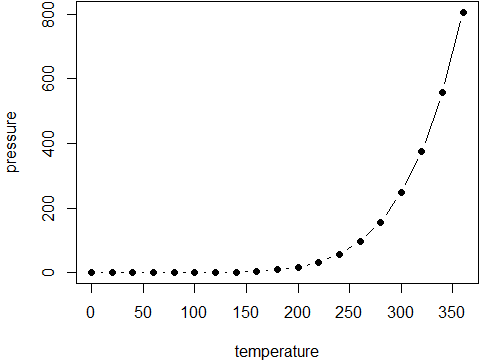
\includegraphics[width=0.8\linewidth,alt={Plot with connected points showing that vapor pressure of mercury increases exponentially as temperature increases.}]{Chap3_files/figure-latex/nice-fig-1} 

}

\caption{Here is a nice figure!}\label{fig:nice-fig}
\end{figure}

Don't miss Table \ref{tab:nice-tab}.

\begin{Shaded}
\begin{Highlighting}[]
\NormalTok{knitr}\SpecialCharTok{::}\FunctionTok{kable}\NormalTok{(}
  \FunctionTok{head}\NormalTok{(pressure, }\DecValTok{10}\NormalTok{), }\AttributeTok{caption =} \StringTok{\textquotesingle{}Here is a nice table!\textquotesingle{}}\NormalTok{,}
  \AttributeTok{booktabs =} \ConstantTok{TRUE}
\NormalTok{)}
\end{Highlighting}
\end{Shaded}

\begin{table}

\caption{\label{tab:nice-tab}Here is a nice table!}
\centering
\begin{tabular}[t]{rr}
\toprule
temperature & pressure\\
\midrule
0 & 0.0002\\
20 & 0.0012\\
40 & 0.0060\\
60 & 0.0300\\
80 & 0.0900\\
\addlinespace
100 & 0.2700\\
120 & 0.7500\\
140 & 1.8500\\
160 & 4.2000\\
180 & 8.8000\\
\bottomrule
\end{tabular}
\end{table}

\hypertarget{parts}{%
\chapter{Parts}\label{parts}}

You can add parts to organize one or more book chapters together. Parts can be inserted at the top of an .Rmd file, before the first-level chapter heading in that same file.

Add a numbered part: \texttt{\#\ (PART)\ Act\ one\ \{-\}} (followed by \texttt{\#\ A\ chapter})

Add an unnumbered part: \texttt{\#\ (PART\textbackslash{}*)\ Act\ one\ \{-\}} (followed by \texttt{\#\ A\ chapter})

Add an appendix as a special kind of un-numbered part: \texttt{\#\ (APPENDIX)\ Other\ stuff\ \{-\}} (followed by \texttt{\#\ A\ chapter}). Chapters in an appendix are prepended with letters instead of numbers.

\hypertarget{footnotes-and-citations}{%
\chapter{Footnotes and citations}\label{footnotes-and-citations}}

\hypertarget{footnotes}{%
\section{Footnotes}\label{footnotes}}

Footnotes are put inside the square brackets after a caret \texttt{\^{}{[}{]}}. Like this one \footnote{This is a footnote.}.

\hypertarget{citations}{%
\section{Citations}\label{citations}}

Reference items in your bibliography file(s) using \texttt{@key}.

For example, we are using the \textbf{bookdown} package \citep{R-bookdown} (check out the last code chunk in index.Rmd to see how this citation key was added) in this sample book, which was built on top of R Markdown and \textbf{knitr} \citep{xie2015} (this citation was added manually in an external file book.bib).
Note that the \texttt{.bib} files need to be listed in the index.Rmd with the YAML \texttt{bibliography} key.

The \texttt{bs4\_book} theme makes footnotes appear inline when you click on them. In this example book, we added \texttt{csl:\ chicago-fullnote-bibliography.csl} to the \texttt{index.Rmd} YAML, and include the \texttt{.csl} file. To download a new style, we recommend: \url{https://www.zotero.org/styles/}

The RStudio Visual Markdown Editor can also make it easier to insert citations: \url{https://rstudio.github.io/visual-markdown-editing/\#/citations}

\hypertarget{blocks}{%
\chapter{Blocks}\label{blocks}}

\hypertarget{equations}{%
\section{Equations}\label{equations}}

Here is an equation.

\begin{equation} 
  f\left(k\right) = \binom{n}{k} p^k\left(1-p\right)^{n-k}
  \label{eq:binom}
\end{equation}

You may refer to using \texttt{\textbackslash{}@ref(eq:binom)}, like see Equation \eqref{eq:binom}.

\hypertarget{theorems-and-proofs}{%
\section{Theorems and proofs}\label{theorems-and-proofs}}

Labeled theorems can be referenced in text using \texttt{\textbackslash{}@ref(thm:tri)}, for example, check out this smart theorem \ref{thm:tri}.

\begin{theorem}
\protect\hypertarget{thm:tri}{}\label{thm:tri}For a right triangle, if \(c\) denotes the \emph{length} of the hypotenuse
and \(a\) and \(b\) denote the lengths of the \textbf{other} two sides, we have
\[a^2 + b^2 = c^2\]
\end{theorem}

Read more here \url{https://bookdown.org/yihui/bookdown/markdown-extensions-by-bookdown.html}.

\hypertarget{callout-blocks}{%
\section{Callout blocks}\label{callout-blocks}}

The \texttt{bs4\_book} theme also includes special callout blocks, like this \texttt{.rmdnote}.

You can use \textbf{markdown} inside a block.

\begin{Shaded}
\begin{Highlighting}[]
\FunctionTok{head}\NormalTok{(beaver1, }\AttributeTok{n =} \DecValTok{5}\NormalTok{)}
\CommentTok{\#\textgreater{}   day time  temp activ}
\CommentTok{\#\textgreater{} 1 346  840 36.33     0}
\CommentTok{\#\textgreater{} 2 346  850 36.34     0}
\CommentTok{\#\textgreater{} 3 346  900 36.35     0}
\CommentTok{\#\textgreater{} 4 346  910 36.42     0}
\CommentTok{\#\textgreater{} 5 346  920 36.55     0}
\end{Highlighting}
\end{Shaded}

It is up to the user to define the appearance of these blocks for LaTeX output.

You may also use: \texttt{.rmdcaution}, \texttt{.rmdimportant}, \texttt{.rmdtip}, or \texttt{.rmdwarning} as the block name.

The R Markdown Cookbook provides more help on how to use custom blocks to design your own callouts: \url{https://bookdown.org/yihui/rmarkdown-cookbook/custom-blocks.html}

\hypertarget{sharing-your-book}{%
\chapter{Sharing your book}\label{sharing-your-book}}

\hypertarget{publishing}{%
\section{Publishing}\label{publishing}}

HTML books can be published online, see: \url{https://bookdown.org/yihui/bookdown/publishing.html}

\hypertarget{pages}{%
\section{404 pages}\label{pages}}

By default, users will be directed to a 404 page if they try to access a webpage that cannot be found. If you'd like to customize your 404 page instead of using the default, you may add either a \texttt{\_404.Rmd} or \texttt{\_404.md} file to your project root and use code and/or Markdown syntax.

\hypertarget{metadata-for-sharing}{%
\section{Metadata for sharing}\label{metadata-for-sharing}}

Bookdown HTML books will provide HTML metadata for social sharing on platforms like Twitter, Facebook, and LinkedIn, using information you provide in the \texttt{index.Rmd} YAML. To setup, set the \texttt{url} for your book and the path to your \texttt{cover-image} file. Your book's \texttt{title} and \texttt{description} are also used.

This \texttt{bs4\_book} provides enhanced metadata for social sharing, so that each chapter shared will have a unique description, auto-generated based on the content.

Specify your book's source repository on GitHub as the \texttt{repo} in the \texttt{\_output.yml} file, which allows users to view each chapter's source file or suggest an edit. Read more about the features of this output format here:

\url{https://pkgs.rstudio.com/bookdown/reference/bs4_book.html}

Or use:

\begin{Shaded}
\begin{Highlighting}[]
\NormalTok{?bookdown}\SpecialCharTok{::}\NormalTok{bs4\_book}
\end{Highlighting}
\end{Shaded}


  \bibliography{book.bib,packages.bib}

\end{document}
